\subsection{Import BioPAX 3 document}
BioPAX level 3 information is fully supported (reaction network, interaction network, pathway structure, annotations).\\\\
\textbf{Plugins$\Rightarrow$BiNoM  I/O$\Rightarrow$Import BioPAX 3 Document from file}\\
The model M-Phase.owl\cite{novak1998model} is uploaded. A dialog window proposes to create three different interfaces to the BioPAX file: reaction network (RN), pathway structure (PS) and protein interaction (PP).
\begin{itemize}
\item Reaction network: M-Phase RN is a representation of the reaction network (figure~\ref{View_BioPAX_of_Novak}).
\item Pathway structure: M-Phase PS represents the pathway hierarchical structure. For this example, we choose to show a more detailed and complete pathway, the apoptosis sub-network extracted from Reactome database (figure~\ref{Apoptosis_pathway_hierarchical_structure}).
\item Protein interaction: M-Phase PP shows which proteins interact with each other.
\end{itemize}
For more details on BioPAX, its interfaces, etc, go to section \ref{Standard_BioPAX_Interfaces}.
\begin{figure}
\centering
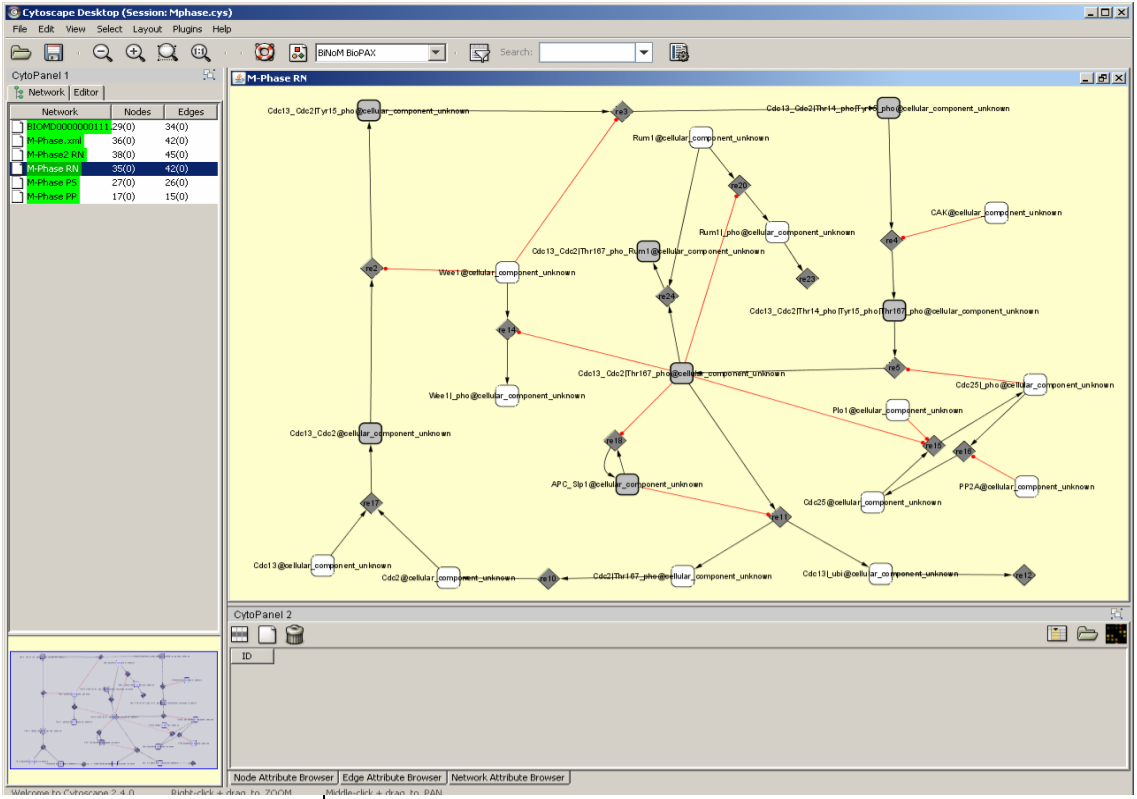
\includegraphics[width=0.8\textwidth]{graphics/View_BioPAX_of_Novak}
\caption{BioPAX view of Novak et al. model.}
\label{View_BioPAX_of_Novak}
\end{figure}
\begin{figure}
\centering
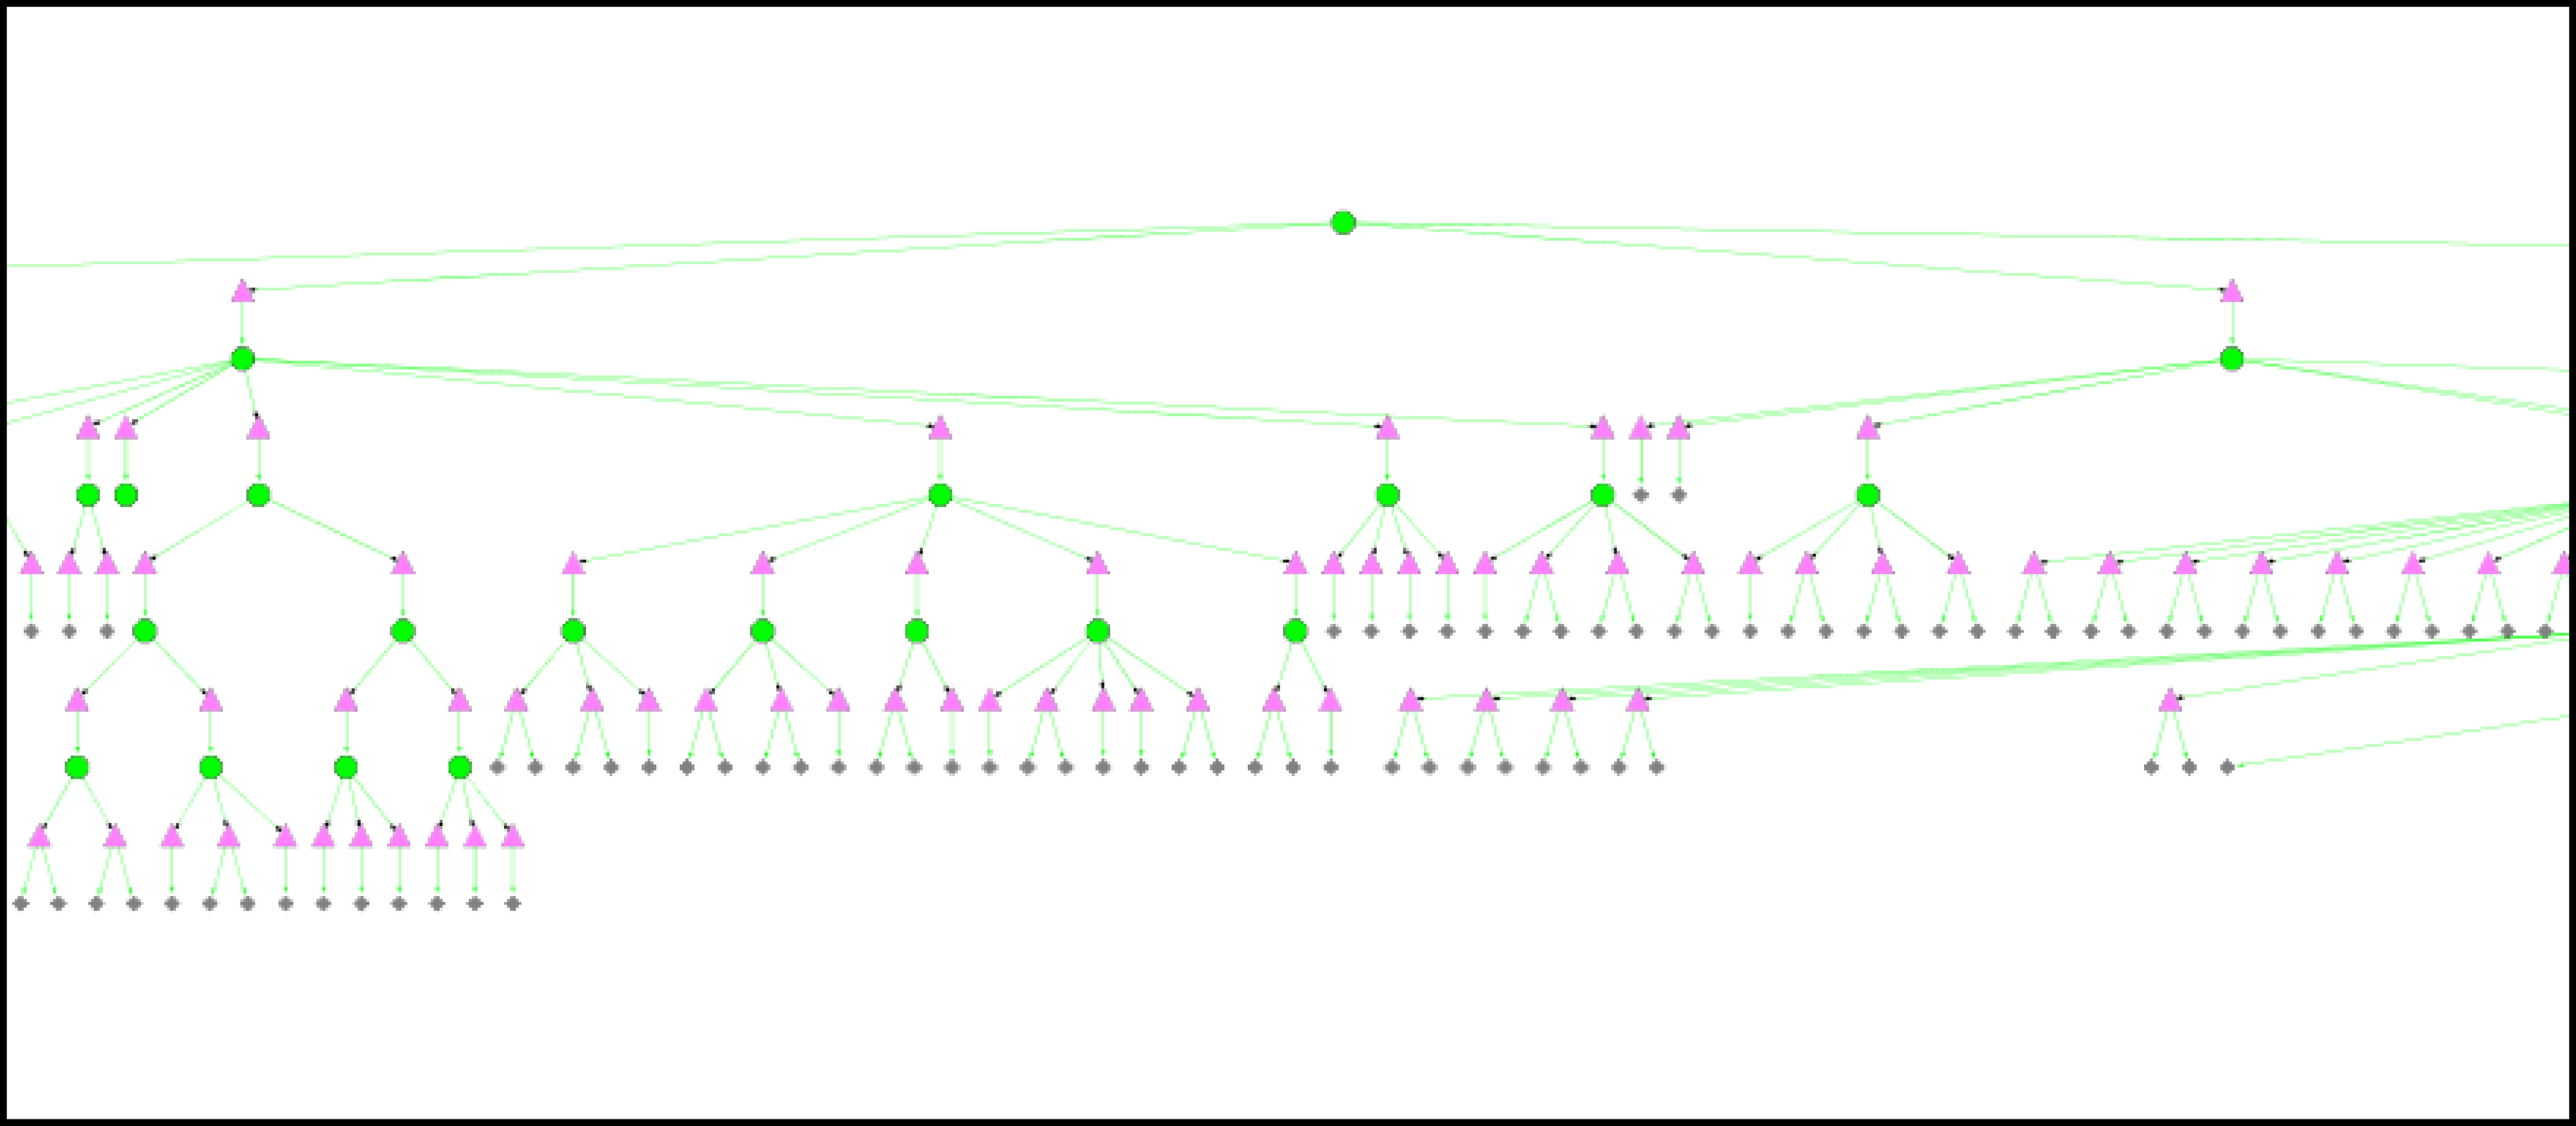
\includegraphics[width=0.8\textwidth]{graphics/Apoptosis_pathway_hierarchical_structure}
\caption{Apoptosis pathway hierarchical structure. Green nodes represent pathways, pink triangular nodes represent steps, and grey nodes represent reactions. From the apoptosis node (top node in red), the cell can choose through 5 different paths. The red-colored path shows one of them, the activation of apoptosis via the intrinsic pathway, leading to the cleavage of caspases 3.}
\label{Apoptosis_pathway_hierarchical_structure}
\end{figure}
\\In the case of creating the pathway structure interface, several choices are offered:
\begin{itemize}
\item Make Root Pathway Node: adds an extra node to which all pathways are connected. This feature can be useful for organizing the graph and joining separate and disjoint pathways.
\item Include Next Links: shows the ‘order’ of the reactions. From a node, an arrow indicates which node is the next step. This feature provides a timeline of the events in a pathway and could emphasize, for example, the linearity of a cascade.
\item Include Pathways: includes green nodes (figure~\ref{Apoptosis_pathway_hierarchical_structure}) which correspond to the names of the different pathways of the network.
\item Include interactions: shows explicitly the reactions involved in the pathway (lower grey nodes in figure~\ref{Apoptosis_pathway_hierarchical_structure}).
\end{itemize}\
\textbf{Plugins$\Rightarrow$BiNoM I/O$\Rightarrow$Import BioPAX 3 Document from URL}\\
A BioPAX 3 document can also be imported directly from a URL. The web address must be typed in the dialog window.

\subsection{Import CellDesigner document}
\textbf{Plugins$\Rightarrow$BiNoM I/O$\Rightarrow$Import CellDesigner Document from file}\\
The model can be drawn – or downloaded\cite{novak1998model} – in CellDesigner (figure~\ref{CellDesigner_view_of_yeast_cell_division}) and saved as M-Phase.xml.\\
The “Import CellDesigner Document from file” function imports a model from CellDesigner to Cytoscape.  A dialog window opens and M-Phase.xml needs to be selected and imported (figure~\ref{Cytoscape_view_of_yeast_cell_division}).\\
\begin{figure}
\centering
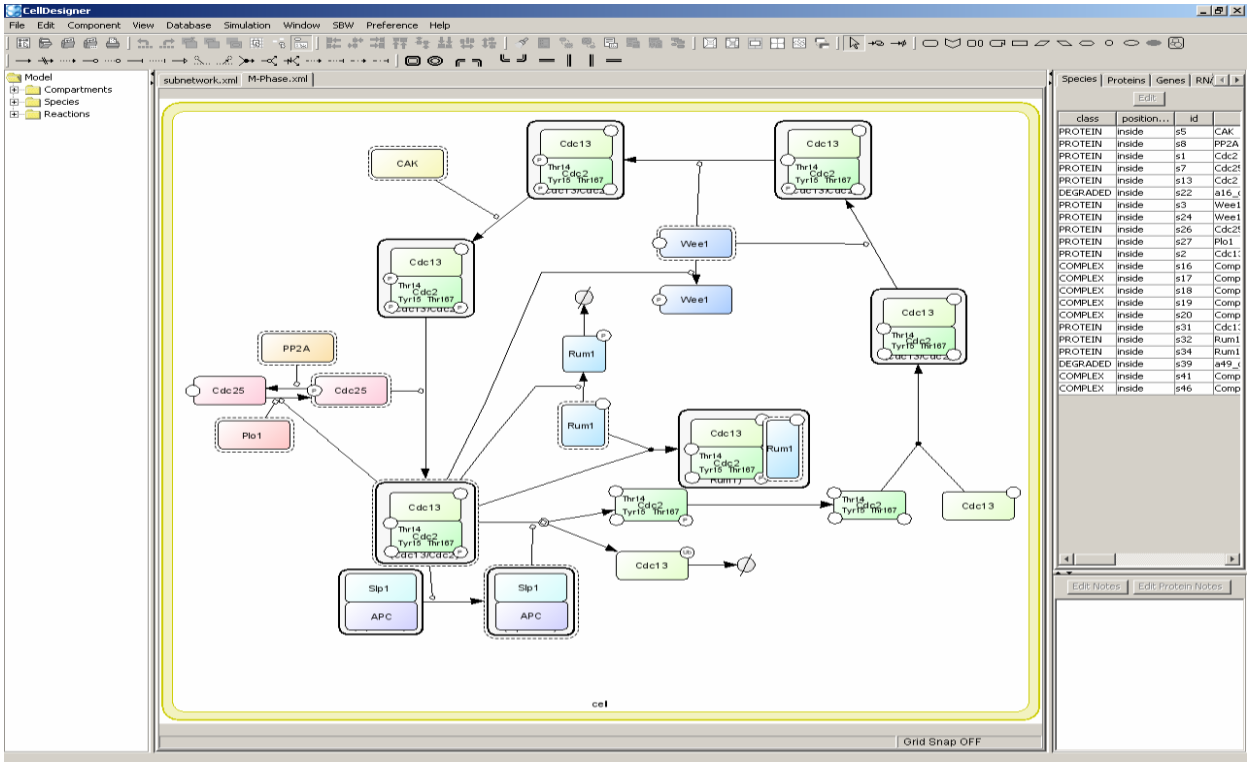
\includegraphics[width=0.8\textwidth]{graphics/CellDesigner_view_of_yeast_cell_division}
\caption{CellDesigner view of the cell division cycle model of fission yeast\cite{novak1998model}}
\label{CellDesigner_view_of_yeast_cell_division}
\end{figure}\begin{figure}
\centering
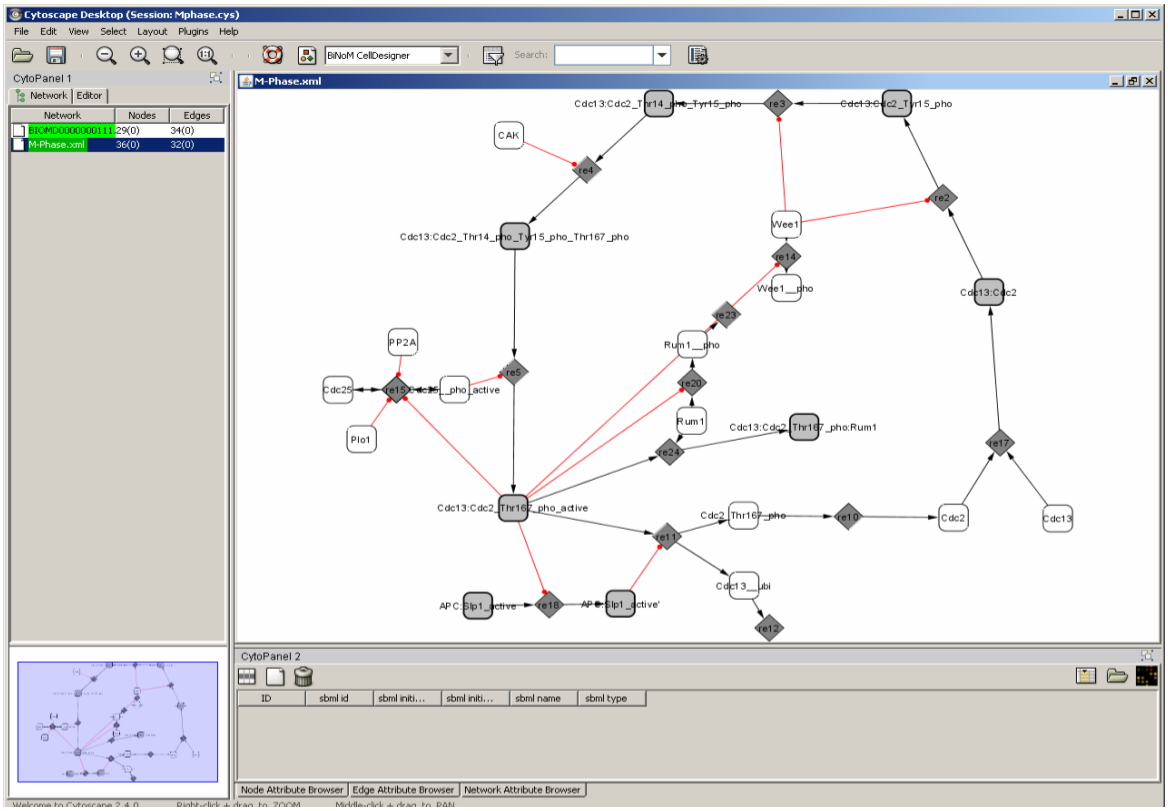
\includegraphics[width=0.8\textwidth]{graphics/Cytoscape_view_of_yeast_cell_division}
\caption{Cytoscape view of the cell division cycle model of fission yeast from a CellDesigner document}
\label{Cytoscape_view_of_yeast_cell_division}
\end{figure}
\\Figure~\ref{CellDesigner_view_of_yeast_cell_division}~and~\ref{Cytoscape_view_of_yeast_cell_division} show the same model viewed by CellDesigner and Cytoscape respectively. The layout information from CellDesigner is imported automatically into Cytoscape.\\\\
In species notes in CellDesigner “Attribute name:Value” as HUGO:E2F1 (without blank) is converted in Cytoscape as the attribute HUGO with the value E2F1 for the specie.\\\\

\subsection{Import CSML document}

\textbf{Plugins$\Rightarrow$BiNoM I/O$\Rightarrow$Import CSML document}\\
BiNoM imports a CSML (Cell System Markup Language, csml.org)

\subsection{Import influence network from AIN file} \label{Import_AIN_file}

\textbf{Plugins$\Rightarrow$BiNoM I/O$\Rightarrow$Import AIN file}\\

This option proposes to automatically import an influence network in Cytoscape
from a simple tab-delimited text file. We call the format of the
text file AIN (Annotated Influence Network). Basically each row of the text file is encoding an
interaction between two species, with a few optional descriptive fields. The precise
format for each field is described in the appendices (section~\ref{AIN_file_format}). 

The AIN file of the apoptosis model ExamplApop.txt is imported. First, the user
is asked to manage the families (groups of genes or proteins, see the appendices
for a precise description): they can be expanded (replacing the family by all
its members) or collapsed (replacing all family members by the name of the
family). See figure~\ref{AIN_dialog_for_families_management}.\\\\

\begin{figure}
\centering
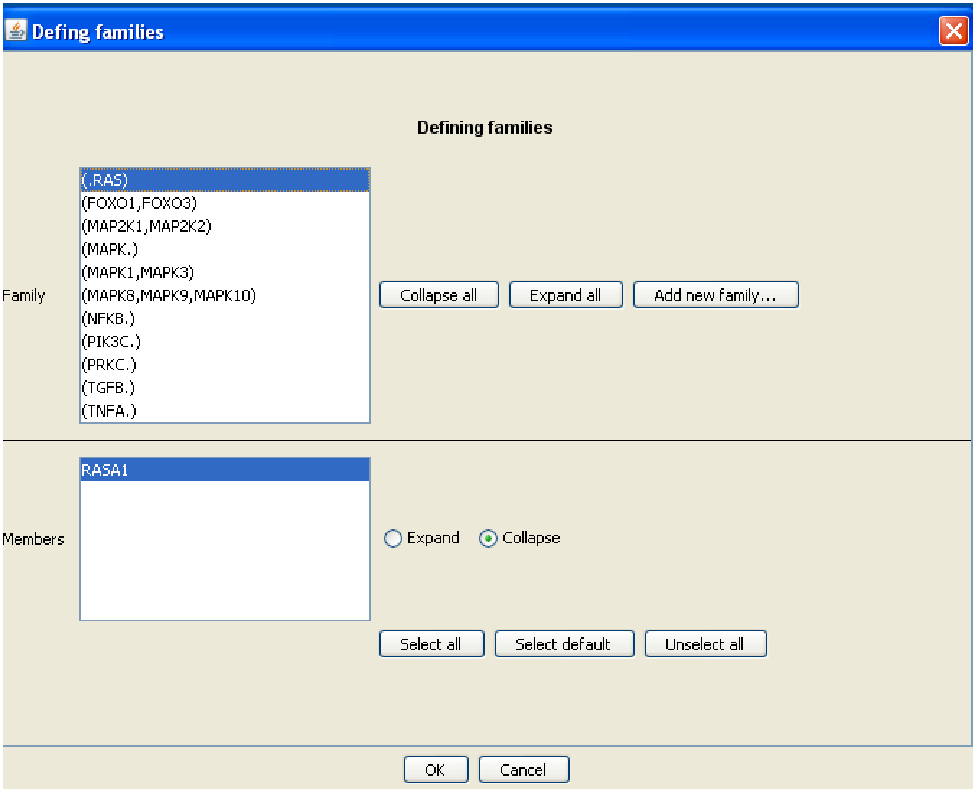
\includegraphics[width=0.8\textwidth]{graphics/AIN_dialog_for_families_management}
\caption{Dialog window for families management when importing apoptosis influence file. BiNoM automatically detects gene families and proposes to either collapse or expand them.}
\label{AIN_dialog_for_families_management}
\end{figure}

Then a dialog window proposes to add constitutive reactions: influences that
link proteins (or families) to their complexes and proteins (or families) to
their phosphorylated state. See
figure~\ref{AIN_dialog_for_constitutive_reactions}.\\\\

\begin{figure}
\centering
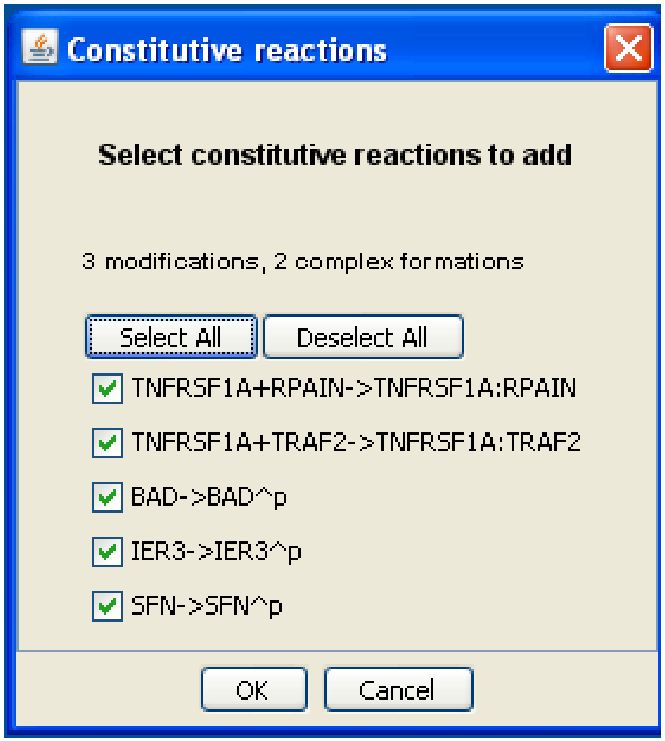
\includegraphics[width=0.5\textwidth]{graphics/AIN_dialog_for_constitutive_reactions}
\caption{Dialog window for constitutive reactions when importing apoptosis influence file. BiNoM detects all possible constitutive reactions and proposes to add them.}
\label{AIN_dialog_for_constitutive_reactions}
\end{figure}
The imported network is synchronized with BioPAX format that includes the annotations of the AIN file. All this information can be accessed via “BioPAX 3 property editor” (see BioPAX Utils, section ~\ref{BioPAX_Property_Editor}).

\subsection{Export current network to BioPAX 3, Export current network to CellDesigner} \label{Export_current_network}
The Cytoscape networks can be exported in BioPAX and CellDesigner by:
\begin{itemize}
\item \textbf{Plugins$\Rightarrow$BiNoM I/O$\Rightarrow$Export current network to BioPAX 3}
\item \textbf{Plugins$\Rightarrow$BiNoM I/O$\Rightarrow$Export current network to CellDesigner}
\end{itemize}
\includegraphics[width=12pt,height=12pt]{graphics/warning} provided that they are associated to existing CellDesigner or BioPAX by:
\begin{itemize}
\item Associate BioPAX Source, see section~\ref{Associate_BioPAX_Source}.
\item Associate CellDesigner Source,see~\ref{Associate_CellDesigner_Source}.
\end{itemize}
More precisely, BiNoM is able to convert CellDesigner to BioPAX, and BioPAX reaction network interface to pure SBML. BiNoM is also able to export only a part of CellDesigner and BioPAX file, visible in the current Cytoscape network (interface). During the export operation, BiNoM is also able to merge a part of associated BioPAX file with already saved another part. BiNoM can modify the content of a BioPAX file. \\\\
\includegraphics[width=12pt,height=12pt]{graphics/warning} BiNoM is NOT able to create CellDesigner file with all graphical notations from BioPAX or from scratch, and it is not able to modify the content of a CellDesigner file.\\\\
Here are the typical scenarios where BiNoM export operations can be useful.
\begin{enumerate}
\item User imports a big BioPAX file as reaction network and using Cytoscape creates a new subnetwork from the global reaction graph. After he can export this subnetwork into a separate self-containing BioPAX file.
\item User imports the pathway structure of a big BioPAX file and selects only a few pathway or pathwayStep nodes he is interested in. After he can export a part of the BioPAX file necessary to define these pathways.
\item User imports a BioPAX file as reaction network, selects a subnetwork and exports it as pure SBML to be used for creation of a computational model of this subpart later.
\item User imports CellDesigner file, selects a subnetwork and exports it as a CellDesigner file: it can be useful for creating a CellDesigner image of a network module of a big reaction network.
\item User imports CellDesigner file, selects a subnetwork and exports it as a BioPAX file (some SBML-specific information such as parameters values will be lost).
\end{enumerate}
The networks created as a result of the import operation are already associated to the corresponding BioPAX or CellDesigner files. However, if the XGMML file is saved and used in another Cytoscape session, or if a new network is created from the initial network with Cytoscape New menu then this association is lost.\\\\
To perform export operation, the network should be Re-associated to the corresponding file (from which it is originated) through Plugins$\Rightarrow$BiNoM I/O$\Rightarrow$Associate$\ldots$ operation. For huge BioPAX files the association might take some time for the first association, but once the file is loaded into memory cache, the following associations are almost instantaneous.\\\\
To understand better what BiNoM can do or can not, read the sections \ref{Attributed_graph_model}, \ref{BiNoM_Naming_Service} and \ref{Standard_BioPAX_Interfaces} about the BiNoM data model.

\subsection{Export current network to SBML}
\textbf{Plugins$\Rightarrow$BiNoM I/O$\Rightarrow$Export current network to SBML}\\
Export the current network to pure SBML level 2.

\subsection{Associate BioPAX 3 Source} \label{Associate_BioPAX_Source}
\textbf{Plugins$\Rightarrow$BiNoM I/O$\Rightarrow$Associate BioPAX 3 Source}\\
Associate a BioPAX 3 Source to allow exportation in BioPAX 3 as explained in section~\ref{Export_current_network}

\subsection{Save whole associate BioPAX 3 as}
When the content of the BioPAX file is modified (through BioPAX property editor, see section ~\ref{BioPAX_Property_Editor}), it can be to be saved as a whole (not only visible part) by\\
\textbf{Plugins$\Rightarrow$BiNoM I/O$\Rightarrow$Save whole associated BioPAX 3 as}\\
Otherwise, all modifications made in the different interfaces are lost. Changes are visible but only recorded permanently when the document is save.

\subsection{Associate CellDesigner Source}\label{Associate_CellDesigner_Source}
\textbf{Plugins$\Rightarrow$BiNoM I/O$\Rightarrow$Associate BioPAX 3 Source} \\
Associate a CellDesigner Source to allow exportation in CellDesigner as explained in section~\ref{Export_current_network}

\subsection{List all reactions}
\textbf{Plugins$\Rightarrow$BiNoM I/O$\Rightarrow$List all reactions} \\
Display list of reactions, can be copied by control+A then control+C.

\subsection{List all nodes}
\textbf{Plugins$\Rightarrow$BiNoM I/O$\Rightarrow$List all nodes} \\
Display list of nodes, can be copied by control+A then control+C.

\subsection{Color CellDesigner proteins}
\textbf{Plugins$\Rightarrow$BiNoM I/O$\Rightarrow$Color CellDesigner proteins}\\
Cytoscape allows coloring nodes according to values of attributes (for example expression data) by the powerful possibilities of VizMapper. The export to CellDesigner keeps the colors. This process can be used to color species in CellDesigner. The function Color CellDesigner proteins allows to color proteins in CellDesigner which describe the components of complexes.\\\\
The gene expression file is based on Hugo names, data in columns (first line title and tabulation as column separator):\\Hugo names\textless Tab\textgreater expression level 1\textless Tab\textgreater expression level 2$\ldots$\\\\
Open dialog box “Color CellDesigner proteins…”, input CellDesigner file name and gene expression file, click on ok. BiNoM generate a file *.conv where Hugo names are converted in protein names (links by annotation in CellDesigner, check if correct) and a CellDesigner file by column. When there are several Hugo name the highest is kept.\\\\
Figure~\ref{Colored_CellDesigner_view_by_ficticious_data} shows the aspect of colored proteins inside complexes.
\begin{figure}
\centering
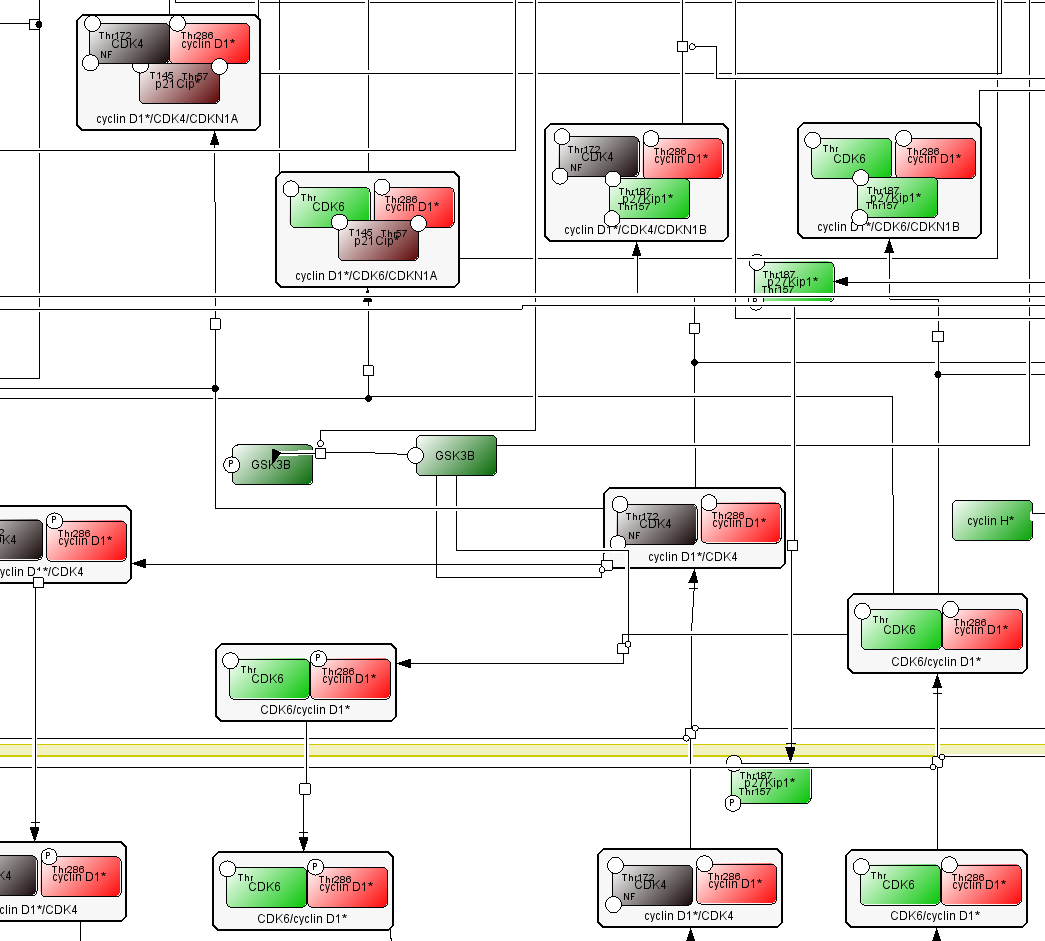
\includegraphics[width=0.8\textwidth]{graphics/Colored_CellDesigner_view_by_ficticious_data}
\caption{CellDesigner view of an extract from Rb-E2F\cite{calzone2008comprehensive} pathway colored by ficticious expression data}
\label{Colored_CellDesigner_view_by_ficticious_data}
\end{figure}

\subsection{Modify CellDesigner notes}
\textbf{Plugins$\Rightarrow$BiNoM I/O$\Rightarrow$Color CellDesigner proteins}\\
Modify in Cytoscape the notes of CellDesigner file when exporting.
